\documentclass[]{article}
\usepackage{lmodern}
\usepackage{amssymb,amsmath}
\usepackage{ifxetex,ifluatex}
\usepackage{fixltx2e} % provides \textsubscript
\ifnum 0\ifxetex 1\fi\ifluatex 1\fi=0 % if pdftex
  \usepackage[T1]{fontenc}
  \usepackage[utf8]{inputenc}
\else % if luatex or xelatex
  \ifxetex
    \usepackage{mathspec}
  \else
    \usepackage{fontspec}
  \fi
  \defaultfontfeatures{Ligatures=TeX,Scale=MatchLowercase}
\fi
% use upquote if available, for straight quotes in verbatim environments
\IfFileExists{upquote.sty}{\usepackage{upquote}}{}
% use microtype if available
\IfFileExists{microtype.sty}{%
\usepackage{microtype}
\UseMicrotypeSet[protrusion]{basicmath} % disable protrusion for tt fonts
}{}
\usepackage[margin=1in]{geometry}
\usepackage{hyperref}
\PassOptionsToPackage{usenames,dvipsnames}{color} % color is loaded by hyperref
\hypersetup{unicode=true,
            pdftitle={Module 2: Recommended Exercises - Solution},
            pdfauthor={Martina Hall, Michail Spitieris, Stefanie Muff, Department of Mathematical Sciences, NTNU},
            colorlinks=true,
            linkcolor=Maroon,
            citecolor=Blue,
            urlcolor=blue,
            breaklinks=true}
\urlstyle{same}  % don't use monospace font for urls
\usepackage{color}
\usepackage{fancyvrb}
\newcommand{\VerbBar}{|}
\newcommand{\VERB}{\Verb[commandchars=\\\{\}]}
\DefineVerbatimEnvironment{Highlighting}{Verbatim}{commandchars=\\\{\}}
% Add ',fontsize=\small' for more characters per line
\usepackage{framed}
\definecolor{shadecolor}{RGB}{248,248,248}
\newenvironment{Shaded}{\begin{snugshade}}{\end{snugshade}}
\newcommand{\KeywordTok}[1]{\textcolor[rgb]{0.13,0.29,0.53}{\textbf{#1}}}
\newcommand{\DataTypeTok}[1]{\textcolor[rgb]{0.13,0.29,0.53}{#1}}
\newcommand{\DecValTok}[1]{\textcolor[rgb]{0.00,0.00,0.81}{#1}}
\newcommand{\BaseNTok}[1]{\textcolor[rgb]{0.00,0.00,0.81}{#1}}
\newcommand{\FloatTok}[1]{\textcolor[rgb]{0.00,0.00,0.81}{#1}}
\newcommand{\ConstantTok}[1]{\textcolor[rgb]{0.00,0.00,0.00}{#1}}
\newcommand{\CharTok}[1]{\textcolor[rgb]{0.31,0.60,0.02}{#1}}
\newcommand{\SpecialCharTok}[1]{\textcolor[rgb]{0.00,0.00,0.00}{#1}}
\newcommand{\StringTok}[1]{\textcolor[rgb]{0.31,0.60,0.02}{#1}}
\newcommand{\VerbatimStringTok}[1]{\textcolor[rgb]{0.31,0.60,0.02}{#1}}
\newcommand{\SpecialStringTok}[1]{\textcolor[rgb]{0.31,0.60,0.02}{#1}}
\newcommand{\ImportTok}[1]{#1}
\newcommand{\CommentTok}[1]{\textcolor[rgb]{0.56,0.35,0.01}{\textit{#1}}}
\newcommand{\DocumentationTok}[1]{\textcolor[rgb]{0.56,0.35,0.01}{\textbf{\textit{#1}}}}
\newcommand{\AnnotationTok}[1]{\textcolor[rgb]{0.56,0.35,0.01}{\textbf{\textit{#1}}}}
\newcommand{\CommentVarTok}[1]{\textcolor[rgb]{0.56,0.35,0.01}{\textbf{\textit{#1}}}}
\newcommand{\OtherTok}[1]{\textcolor[rgb]{0.56,0.35,0.01}{#1}}
\newcommand{\FunctionTok}[1]{\textcolor[rgb]{0.00,0.00,0.00}{#1}}
\newcommand{\VariableTok}[1]{\textcolor[rgb]{0.00,0.00,0.00}{#1}}
\newcommand{\ControlFlowTok}[1]{\textcolor[rgb]{0.13,0.29,0.53}{\textbf{#1}}}
\newcommand{\OperatorTok}[1]{\textcolor[rgb]{0.81,0.36,0.00}{\textbf{#1}}}
\newcommand{\BuiltInTok}[1]{#1}
\newcommand{\ExtensionTok}[1]{#1}
\newcommand{\PreprocessorTok}[1]{\textcolor[rgb]{0.56,0.35,0.01}{\textit{#1}}}
\newcommand{\AttributeTok}[1]{\textcolor[rgb]{0.77,0.63,0.00}{#1}}
\newcommand{\RegionMarkerTok}[1]{#1}
\newcommand{\InformationTok}[1]{\textcolor[rgb]{0.56,0.35,0.01}{\textbf{\textit{#1}}}}
\newcommand{\WarningTok}[1]{\textcolor[rgb]{0.56,0.35,0.01}{\textbf{\textit{#1}}}}
\newcommand{\AlertTok}[1]{\textcolor[rgb]{0.94,0.16,0.16}{#1}}
\newcommand{\ErrorTok}[1]{\textcolor[rgb]{0.64,0.00,0.00}{\textbf{#1}}}
\newcommand{\NormalTok}[1]{#1}
\usepackage{graphicx,grffile}
\makeatletter
\def\maxwidth{\ifdim\Gin@nat@width>\linewidth\linewidth\else\Gin@nat@width\fi}
\def\maxheight{\ifdim\Gin@nat@height>\textheight\textheight\else\Gin@nat@height\fi}
\makeatother
% Scale images if necessary, so that they will not overflow the page
% margins by default, and it is still possible to overwrite the defaults
% using explicit options in \includegraphics[width, height, ...]{}
\setkeys{Gin}{width=\maxwidth,height=\maxheight,keepaspectratio}
\IfFileExists{parskip.sty}{%
\usepackage{parskip}
}{% else
\setlength{\parindent}{0pt}
\setlength{\parskip}{6pt plus 2pt minus 1pt}
}
\setlength{\emergencystretch}{3em}  % prevent overfull lines
\providecommand{\tightlist}{%
  \setlength{\itemsep}{0pt}\setlength{\parskip}{0pt}}
\setcounter{secnumdepth}{0}
% Redefines (sub)paragraphs to behave more like sections
\ifx\paragraph\undefined\else
\let\oldparagraph\paragraph
\renewcommand{\paragraph}[1]{\oldparagraph{#1}\mbox{}}
\fi
\ifx\subparagraph\undefined\else
\let\oldsubparagraph\subparagraph
\renewcommand{\subparagraph}[1]{\oldsubparagraph{#1}\mbox{}}
\fi

%%% Use protect on footnotes to avoid problems with footnotes in titles
\let\rmarkdownfootnote\footnote%
\def\footnote{\protect\rmarkdownfootnote}

%%% Change title format to be more compact
\usepackage{titling}

% Create subtitle command for use in maketitle
\providecommand{\subtitle}[1]{
  \posttitle{
    \begin{center}\large#1\end{center}
    }
}

\setlength{\droptitle}{-2em}

  \title{Module 2: Recommended Exercises - Solution}
    \pretitle{\vspace{\droptitle}\centering\huge}
  \posttitle{\par}
  \subtitle{TMA4268 Statistical Learning V2020}
  \author{Martina Hall, Michail Spitieris, Stefanie Muff, Department of
Mathematical Sciences, NTNU}
    \preauthor{\centering\large\emph}
  \postauthor{\par}
      \predate{\centering\large\emph}
  \postdate{\par}
    \date{January 16, 2020}


\begin{document}
\maketitle

Last changes: (10.01.2020)

\begin{center}\rule{0.5\linewidth}{\linethickness}\end{center}

\section{Problem 1 - Classification}\label{problem-1---classification}

Example 1: Cancer diagnostics. Response: cancer (yes/no). Predictors:
smoking, age, family history, gene expression ect. Goal: prediction.
Example 2: Stock market price direction. Response: up/down. Predictors:
yesterday's price movement change, two previous days price movement ect.
Goal: inference. Example 3: Flower specie. Response: specie. Predictors:
color, height, leafes ect. Goal: prediction

\section{Problem 2 - Regression}\label{problem-2---regression}

Example 1: Illness classification. Response: age of death. Predictors:
current age, gender, resting heart rate, resting breath rate ect. Goal:
prediction Example 2: House price. Response: Price. Predictors: age of
house, price of neighbourhood, crime rate, distance to town, distance to
school, ect. Goal: prediction Example 3: What affects O2-uptake.
Response: O2-uptake. Predictors: gender, age, amount of weekly exercise,
type of exercise, smoking, heart disease, ect. Goal: inference

\section{Problem 3}\label{problem-3}

\begin{enumerate}
\def\labelenumi{\alph{enumi})}
\tightlist
\item
  A rigid method will typically have the highest test error.
\item
  A small (test) variance imply an underfit to the data.
\item
  See figure 2.12. Underfit - low variance - high bias. Overfit - high
  variance - low bias. We wish to find a model that lies somewhere
  inbetween, with low variance and low bias.
\end{enumerate}

\section{Problem 4}\label{problem-4}

\begin{Shaded}
\begin{Highlighting}[]
\CommentTok{#install.packages("ISLR")}
\KeywordTok{library}\NormalTok{(ISLR)}
\KeywordTok{data}\NormalTok{(Auto)}
\end{Highlighting}
\end{Shaded}

\begin{enumerate}
\def\labelenumi{\alph{enumi})}
\item
\end{enumerate}

\begin{Shaded}
\begin{Highlighting}[]
\CommentTok{#a)}
\KeywordTok{str}\NormalTok{(Auto)}
\end{Highlighting}
\end{Shaded}

\begin{verbatim}
## 'data.frame':    392 obs. of  9 variables:
##  $ mpg         : num  18 15 18 16 17 15 14 14 14 15 ...
##  $ cylinders   : num  8 8 8 8 8 8 8 8 8 8 ...
##  $ displacement: num  307 350 318 304 302 429 454 440 455 390 ...
##  $ horsepower  : num  130 165 150 150 140 198 220 215 225 190 ...
##  $ weight      : num  3504 3693 3436 3433 3449 ...
##  $ acceleration: num  12 11.5 11 12 10.5 10 9 8.5 10 8.5 ...
##  $ year        : num  70 70 70 70 70 70 70 70 70 70 ...
##  $ origin      : num  1 1 1 1 1 1 1 1 1 1 ...
##  $ name        : Factor w/ 304 levels "amc ambassador brougham",..: 49 36 231 14 161 141 54 223 241 2 ...
\end{verbatim}

\begin{Shaded}
\begin{Highlighting}[]
\KeywordTok{summary}\NormalTok{(Auto)}
\end{Highlighting}
\end{Shaded}

\begin{verbatim}
##       mpg          cylinders      displacement     horsepower   
##  Min.   : 9.00   Min.   :3.000   Min.   : 68.0   Min.   : 46.0  
##  1st Qu.:17.00   1st Qu.:4.000   1st Qu.:105.0   1st Qu.: 75.0  
##  Median :22.75   Median :4.000   Median :151.0   Median : 93.5  
##  Mean   :23.45   Mean   :5.472   Mean   :194.4   Mean   :104.5  
##  3rd Qu.:29.00   3rd Qu.:8.000   3rd Qu.:275.8   3rd Qu.:126.0  
##  Max.   :46.60   Max.   :8.000   Max.   :455.0   Max.   :230.0  
##                                                                 
##      weight      acceleration        year           origin     
##  Min.   :1613   Min.   : 8.00   Min.   :70.00   Min.   :1.000  
##  1st Qu.:2225   1st Qu.:13.78   1st Qu.:73.00   1st Qu.:1.000  
##  Median :2804   Median :15.50   Median :76.00   Median :1.000  
##  Mean   :2978   Mean   :15.54   Mean   :75.98   Mean   :1.577  
##  3rd Qu.:3615   3rd Qu.:17.02   3rd Qu.:79.00   3rd Qu.:2.000  
##  Max.   :5140   Max.   :24.80   Max.   :82.00   Max.   :3.000  
##                                                                
##                  name    
##  amc matador       :  5  
##  ford pinto        :  5  
##  toyota corolla    :  5  
##  amc gremlin       :  4  
##  amc hornet        :  4  
##  chevrolet chevette:  4  
##  (Other)           :365
\end{verbatim}

See from looking at the structure (\texttt{str()}) and
\texttt{summary()} that cylinders (taking values 3,4,5,6,8), origin
(taking values 1,2,3) and name (name of the cars) are qualitative
predictors. The rest of the predictors are quantitative.

\begin{enumerate}
\def\labelenumi{\alph{enumi})}
\setcounter{enumi}{1}
\tightlist
\item
  To see the range of the quantitative predictors, either apply the
  \texttt{range()} function to each column with a quantitative predictor
  separately
\end{enumerate}

\begin{Shaded}
\begin{Highlighting}[]
\KeywordTok{range}\NormalTok{(Auto[,}\DecValTok{1}\NormalTok{])}
\end{Highlighting}
\end{Shaded}

\begin{verbatim}
## [1]  9.0 46.6
\end{verbatim}

\begin{Shaded}
\begin{Highlighting}[]
\KeywordTok{range}\NormalTok{(Auto[,}\DecValTok{3}\NormalTok{])}
\end{Highlighting}
\end{Shaded}

\begin{verbatim}
## [1]  68 455
\end{verbatim}

\begin{Shaded}
\begin{Highlighting}[]
\KeywordTok{range}\NormalTok{(Auto[,}\DecValTok{4}\NormalTok{])}
\end{Highlighting}
\end{Shaded}

\begin{verbatim}
## [1]  46 230
\end{verbatim}

\begin{Shaded}
\begin{Highlighting}[]
\KeywordTok{range}\NormalTok{(Auto[,}\DecValTok{5}\NormalTok{])}
\end{Highlighting}
\end{Shaded}

\begin{verbatim}
## [1] 1613 5140
\end{verbatim}

\begin{Shaded}
\begin{Highlighting}[]
\KeywordTok{range}\NormalTok{(Auto[,}\DecValTok{6}\NormalTok{])}
\end{Highlighting}
\end{Shaded}

\begin{verbatim}
## [1]  8.0 24.8
\end{verbatim}

\begin{Shaded}
\begin{Highlighting}[]
\KeywordTok{range}\NormalTok{(Auto[,}\DecValTok{7}\NormalTok{])}
\end{Highlighting}
\end{Shaded}

\begin{verbatim}
## [1] 70 82
\end{verbatim}

or use the \texttt{sapply()} function to run the \texttt{range()}
function on the specified columns with a single line of code:

\begin{Shaded}
\begin{Highlighting}[]
\NormalTok{quant =}\StringTok{ }\KeywordTok{c}\NormalTok{(}\DecValTok{1}\NormalTok{,}\DecValTok{3}\NormalTok{,}\DecValTok{4}\NormalTok{,}\DecValTok{5}\NormalTok{,}\DecValTok{6}\NormalTok{,}\DecValTok{7}\NormalTok{)}
\KeywordTok{sapply}\NormalTok{(Auto[, quant], range)}
\end{Highlighting}
\end{Shaded}

\begin{verbatim}
##       mpg displacement horsepower weight acceleration year
## [1,]  9.0           68         46   1613          8.0   70
## [2,] 46.6          455        230   5140         24.8   82
\end{verbatim}

\begin{enumerate}
\def\labelenumi{\alph{enumi})}
\setcounter{enumi}{2}
\tightlist
\item
  To get the and standard deviation of the quantitative predictors, we
  can again either use the \texttt{sapply()} function in the same manner
  as above, or apply the \texttt{mean()} and \texttt{sd()} commands
  columnwise.
\end{enumerate}

\begin{Shaded}
\begin{Highlighting}[]
\CommentTok{#mean}
\KeywordTok{sapply}\NormalTok{(Auto[, quant], mean)}
\end{Highlighting}
\end{Shaded}

\begin{verbatim}
##          mpg displacement   horsepower       weight acceleration 
##     23.44592    194.41199    104.46939   2977.58418     15.54133 
##         year 
##     75.97959
\end{verbatim}

\begin{Shaded}
\begin{Highlighting}[]
\CommentTok{#or}
\KeywordTok{mean}\NormalTok{(Auto[,}\DecValTok{1}\NormalTok{])}
\end{Highlighting}
\end{Shaded}

\begin{verbatim}
## [1] 23.44592
\end{verbatim}

\begin{Shaded}
\begin{Highlighting}[]
\KeywordTok{mean}\NormalTok{(Auto[,}\DecValTok{3}\NormalTok{])}
\end{Highlighting}
\end{Shaded}

\begin{verbatim}
## [1] 194.412
\end{verbatim}

\begin{Shaded}
\begin{Highlighting}[]
\KeywordTok{mean}\NormalTok{(Auto[,}\DecValTok{4}\NormalTok{])}
\end{Highlighting}
\end{Shaded}

\begin{verbatim}
## [1] 104.4694
\end{verbatim}

\begin{Shaded}
\begin{Highlighting}[]
\KeywordTok{mean}\NormalTok{(Auto[,}\DecValTok{5}\NormalTok{])}
\end{Highlighting}
\end{Shaded}

\begin{verbatim}
## [1] 2977.584
\end{verbatim}

\begin{Shaded}
\begin{Highlighting}[]
\KeywordTok{mean}\NormalTok{(Auto[,}\DecValTok{6}\NormalTok{])}
\end{Highlighting}
\end{Shaded}

\begin{verbatim}
## [1] 15.54133
\end{verbatim}

\begin{Shaded}
\begin{Highlighting}[]
\KeywordTok{mean}\NormalTok{(Auto[,}\DecValTok{7}\NormalTok{])}
\end{Highlighting}
\end{Shaded}

\begin{verbatim}
## [1] 75.97959
\end{verbatim}

\begin{Shaded}
\begin{Highlighting}[]
\CommentTok{#or}
\KeywordTok{colMeans}\NormalTok{(Auto[,quant])}
\end{Highlighting}
\end{Shaded}

\begin{verbatim}
##          mpg displacement   horsepower       weight acceleration 
##     23.44592    194.41199    104.46939   2977.58418     15.54133 
##         year 
##     75.97959
\end{verbatim}

\begin{Shaded}
\begin{Highlighting}[]
\CommentTok{#sd}
\KeywordTok{sapply}\NormalTok{(Auto[, quant], sd)}
\end{Highlighting}
\end{Shaded}

\begin{verbatim}
##          mpg displacement   horsepower       weight acceleration 
##     7.805007   104.644004    38.491160   849.402560     2.758864 
##         year 
##     3.683737
\end{verbatim}

\begin{Shaded}
\begin{Highlighting}[]
\CommentTok{#or}
\KeywordTok{sd}\NormalTok{(Auto[,}\DecValTok{1}\NormalTok{])}
\end{Highlighting}
\end{Shaded}

\begin{verbatim}
## [1] 7.805007
\end{verbatim}

\begin{Shaded}
\begin{Highlighting}[]
\KeywordTok{sd}\NormalTok{(Auto[,}\DecValTok{3}\NormalTok{])}
\end{Highlighting}
\end{Shaded}

\begin{verbatim}
## [1] 104.644
\end{verbatim}

\begin{Shaded}
\begin{Highlighting}[]
\KeywordTok{sd}\NormalTok{(Auto[,}\DecValTok{4}\NormalTok{])}
\end{Highlighting}
\end{Shaded}

\begin{verbatim}
## [1] 38.49116
\end{verbatim}

\begin{Shaded}
\begin{Highlighting}[]
\KeywordTok{sd}\NormalTok{(Auto[,}\DecValTok{5}\NormalTok{])}
\end{Highlighting}
\end{Shaded}

\begin{verbatim}
## [1] 849.4026
\end{verbatim}

\begin{Shaded}
\begin{Highlighting}[]
\KeywordTok{sd}\NormalTok{(Auto[,}\DecValTok{6}\NormalTok{])}
\end{Highlighting}
\end{Shaded}

\begin{verbatim}
## [1] 2.758864
\end{verbatim}

\begin{Shaded}
\begin{Highlighting}[]
\KeywordTok{sd}\NormalTok{(Auto[,}\DecValTok{7}\NormalTok{])}
\end{Highlighting}
\end{Shaded}

\begin{verbatim}
## [1] 3.683737
\end{verbatim}

\begin{enumerate}
\def\labelenumi{\alph{enumi})}
\setcounter{enumi}{3}
\tightlist
\item
  Remove 10th to 85th observations and look at the range, mean and
  standard deviation of the reduced set. We now only show the solutions
  using \texttt{sapply()} to save space.
\end{enumerate}

\begin{Shaded}
\begin{Highlighting}[]
\CommentTok{#remove observations}
\NormalTok{ReducedAuto =}\StringTok{ }\NormalTok{Auto[}\OperatorTok{-}\KeywordTok{c}\NormalTok{(}\DecValTok{10}\OperatorTok{:}\DecValTok{85}\NormalTok{),]}

\CommentTok{#range, mean and sd}
\KeywordTok{sapply}\NormalTok{(ReducedAuto[, quant], range)}
\end{Highlighting}
\end{Shaded}

\begin{verbatim}
##       mpg displacement horsepower weight acceleration year
## [1,] 11.0           68         46   1649          8.5   70
## [2,] 46.6          455        230   4997         24.8   82
\end{verbatim}

\begin{Shaded}
\begin{Highlighting}[]
\KeywordTok{sapply}\NormalTok{(ReducedAuto[, quant], mean)}
\end{Highlighting}
\end{Shaded}

\begin{verbatim}
##          mpg displacement   horsepower       weight acceleration 
##     24.40443    187.24051    100.72152   2935.97152     15.72690 
##         year 
##     77.14557
\end{verbatim}

\begin{Shaded}
\begin{Highlighting}[]
\KeywordTok{sapply}\NormalTok{(ReducedAuto[, quant], sd)}
\end{Highlighting}
\end{Shaded}

\begin{verbatim}
##          mpg displacement   horsepower       weight acceleration 
##     7.867283    99.678367    35.708853   811.300208     2.693721 
##         year 
##     3.106217
\end{verbatim}

\begin{enumerate}
\def\labelenumi{\alph{enumi})}
\setcounter{enumi}{4}
\tightlist
\item
  Make a scatterplot of the full dataset using the \texttt{ggpairs()}
  function.
\end{enumerate}

\begin{Shaded}
\begin{Highlighting}[]
\KeywordTok{library}\NormalTok{(GGally)}
\end{Highlighting}
\end{Shaded}

\begin{verbatim}
## Loading required package: ggplot2
\end{verbatim}

\begin{verbatim}
## Registered S3 method overwritten by 'GGally':
##   method from   
##   +.gg   ggplot2
\end{verbatim}

\begin{Shaded}
\begin{Highlighting}[]
\KeywordTok{ggpairs}\NormalTok{(Auto[,quant]) }\OperatorTok{+}\StringTok{ }\KeywordTok{theme_minimal}\NormalTok{()}
\end{Highlighting}
\end{Shaded}

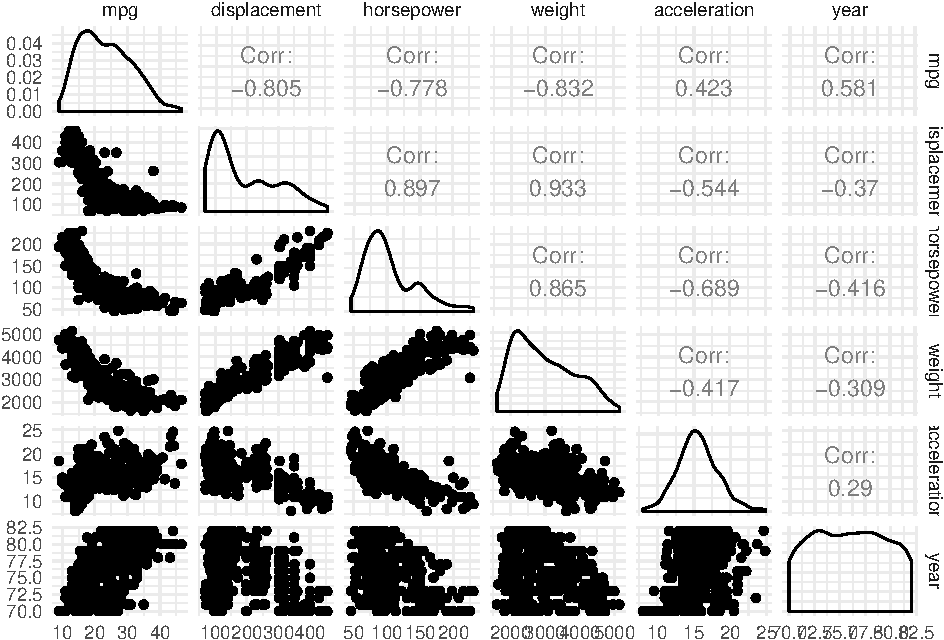
\includegraphics{RecEx2-sol_files/figure-latex/unnamed-chunk-7-1.pdf}

We see that there seems to be strong relationships (based on curve
trends and correlation) between the pairs: \texttt{mpg} and
\texttt{displacement}, \texttt{mpg} and \texttt{horsepower},
\texttt{mpg} and \texttt{weight}, \texttt{displacement} and
\texttt{horsepower}, \texttt{displacement} and \texttt{weight},
\texttt{horsepower} and \texttt{weght}, and \texttt{horsepower} and
\texttt{acceleration}.

\begin{enumerate}
\def\labelenumi{\alph{enumi})}
\setcounter{enumi}{5}
\tightlist
\item
  Wish to predict gas milage based on the other variables. From the
  scatterplot we see that \texttt{displacement}, \texttt{horsepower} and
  \texttt{weight} could be good choises for prediction of \texttt{mpg}.
  Check if the qualitative predictors could also be good choises by
  plotting them against \texttt{mpg}.
\end{enumerate}

\begin{Shaded}
\begin{Highlighting}[]
\KeywordTok{ggplot}\NormalTok{(Auto, }\KeywordTok{aes}\NormalTok{(}\KeywordTok{as.factor}\NormalTok{(cylinders), mpg)) }\OperatorTok{+}\StringTok{ }\KeywordTok{geom_boxplot}\NormalTok{(}\DataTypeTok{fill=}\StringTok{"skyblue"}\NormalTok{) }\OperatorTok{+}\StringTok{ }\KeywordTok{labs}\NormalTok{(}\DataTypeTok{title =} \StringTok{"mgp vs cylinders"}\NormalTok{) }
\end{Highlighting}
\end{Shaded}

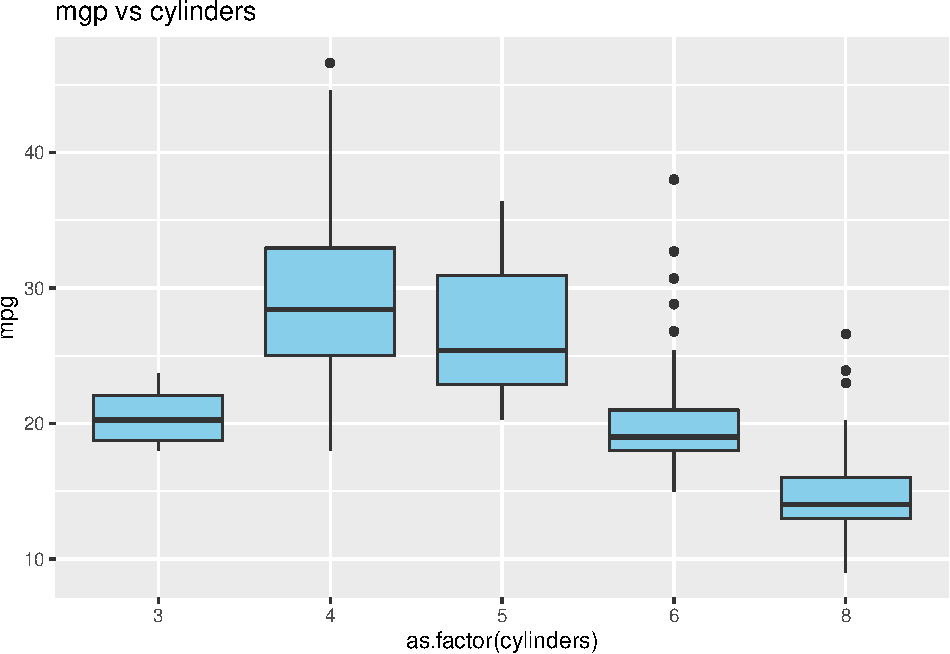
\includegraphics{RecEx2-sol_files/figure-latex/unnamed-chunk-8-1.pdf}

\begin{Shaded}
\begin{Highlighting}[]
\KeywordTok{ggplot}\NormalTok{(Auto, }\KeywordTok{aes}\NormalTok{(}\KeywordTok{as.factor}\NormalTok{(origin), mpg)) }\OperatorTok{+}\StringTok{ }\KeywordTok{geom_boxplot}\NormalTok{(}\DataTypeTok{fill=}\StringTok{"skyblue"}\NormalTok{) }\OperatorTok{+}\StringTok{ }\KeywordTok{labs}\NormalTok{(}\DataTypeTok{title =} \StringTok{"mgp vs origin"}\NormalTok{) }
\end{Highlighting}
\end{Shaded}

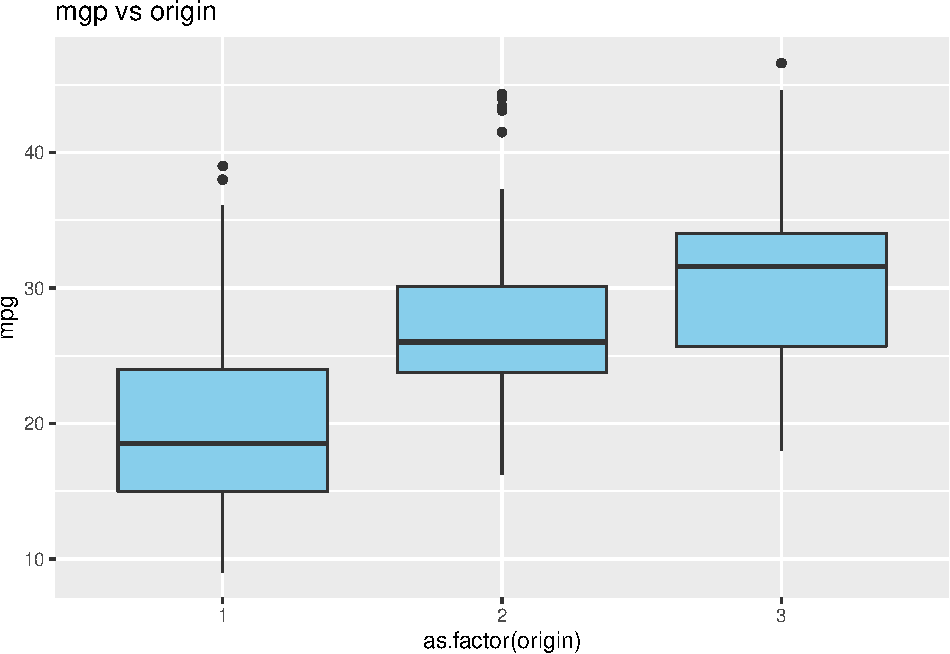
\includegraphics{RecEx2-sol_files/figure-latex/unnamed-chunk-8-2.pdf}

From these plots we see that both \texttt{cylinders} and \texttt{origin}
could be good choices for prediction of \texttt{mgp}, because the miles
per gallon (mpg) seems to depend on these two variables.

\begin{enumerate}
\def\labelenumi{\alph{enumi})}
\setcounter{enumi}{6}
\tightlist
\item
  To find the correlation of the given variables, we need the covariance
  of these variable as well as the standard deviations, which are both
  available in the covariance matrix. Remember the the variance of each
  variable is given in the diagonal of the covariance matrix.
\end{enumerate}

\begin{Shaded}
\begin{Highlighting}[]
\NormalTok{covMat =}\StringTok{ }\KeywordTok{cov}\NormalTok{(Auto[,quant])}
\NormalTok{covMat[}\DecValTok{1}\NormalTok{,}\DecValTok{2}\NormalTok{]}\OperatorTok{/}\NormalTok{(}\KeywordTok{sqrt}\NormalTok{(covMat[}\DecValTok{1}\NormalTok{,}\DecValTok{1}\NormalTok{])}\OperatorTok{*}\KeywordTok{sqrt}\NormalTok{(covMat[}\DecValTok{2}\NormalTok{,}\DecValTok{2}\NormalTok{]))}
\end{Highlighting}
\end{Shaded}

\begin{verbatim}
## [1] -0.8051269
\end{verbatim}

\begin{Shaded}
\begin{Highlighting}[]
\NormalTok{covMat[}\DecValTok{1}\NormalTok{,}\DecValTok{3}\NormalTok{]}\OperatorTok{/}\NormalTok{(}\KeywordTok{sqrt}\NormalTok{(covMat[}\DecValTok{1}\NormalTok{,}\DecValTok{1}\NormalTok{])}\OperatorTok{*}\KeywordTok{sqrt}\NormalTok{(covMat[}\DecValTok{3}\NormalTok{,}\DecValTok{3}\NormalTok{]))}
\end{Highlighting}
\end{Shaded}

\begin{verbatim}
## [1] -0.7784268
\end{verbatim}

\begin{Shaded}
\begin{Highlighting}[]
\NormalTok{covMat[}\DecValTok{1}\NormalTok{,}\DecValTok{4}\NormalTok{]}\OperatorTok{/}\NormalTok{(}\KeywordTok{sqrt}\NormalTok{(covMat[}\DecValTok{1}\NormalTok{,}\DecValTok{1}\NormalTok{])}\OperatorTok{*}\KeywordTok{sqrt}\NormalTok{(covMat[}\DecValTok{4}\NormalTok{,}\DecValTok{4}\NormalTok{]))}
\end{Highlighting}
\end{Shaded}

\begin{verbatim}
## [1] -0.8322442
\end{verbatim}

\begin{Shaded}
\begin{Highlighting}[]
\KeywordTok{cor}\NormalTok{(Auto[,quant])}
\end{Highlighting}
\end{Shaded}

\begin{verbatim}
##                     mpg displacement horsepower     weight acceleration
## mpg           1.0000000   -0.8051269 -0.7784268 -0.8322442    0.4233285
## displacement -0.8051269    1.0000000  0.8972570  0.9329944   -0.5438005
## horsepower   -0.7784268    0.8972570  1.0000000  0.8645377   -0.6891955
## weight       -0.8322442    0.9329944  0.8645377  1.0000000   -0.4168392
## acceleration  0.4233285   -0.5438005 -0.6891955 -0.4168392    1.0000000
## year          0.5805410   -0.3698552 -0.4163615 -0.3091199    0.2903161
##                    year
## mpg           0.5805410
## displacement -0.3698552
## horsepower   -0.4163615
## weight       -0.3091199
## acceleration  0.2903161
## year          1.0000000
\end{verbatim}

We see that the obtained correlations coincide with the given elements
in the correlation matrix.

\section{Problem 5}\label{problem-5}

\begin{enumerate}
\def\labelenumi{\alph{enumi})}
\tightlist
\item
  Simulate values from the four multivariate distributions using
  \texttt{mvnorm()}.
\end{enumerate}

\begin{Shaded}
\begin{Highlighting}[]
\CommentTok{# simulate 1000 values from the multivariate normal distribution with mean = c(2,3) and cov(1,0,0,1)}
\KeywordTok{library}\NormalTok{(MASS)}
\NormalTok{set1 =}\StringTok{ }\KeywordTok{as.data.frame}\NormalTok{(}\KeywordTok{mvrnorm}\NormalTok{(}\DataTypeTok{n =} \DecValTok{1000}\NormalTok{, }\DataTypeTok{mu=}\KeywordTok{c}\NormalTok{(}\DecValTok{2}\NormalTok{,}\DecValTok{3}\NormalTok{), }\DataTypeTok{Sigma =} \KeywordTok{matrix}\NormalTok{(}\KeywordTok{c}\NormalTok{(}\DecValTok{1}\NormalTok{,}\DecValTok{0}\NormalTok{,}\DecValTok{0}\NormalTok{,}\DecValTok{1}\NormalTok{), }\DataTypeTok{ncol=}\DecValTok{2}\NormalTok{)))}
\KeywordTok{colnames}\NormalTok{(set1) =}\StringTok{ }\KeywordTok{c}\NormalTok{(}\StringTok{"x1"}\NormalTok{, }\StringTok{"x2"}\NormalTok{)}

\NormalTok{set2 =}\StringTok{ }\KeywordTok{as.data.frame}\NormalTok{(}\KeywordTok{mvrnorm}\NormalTok{(}\DataTypeTok{n =} \DecValTok{1000}\NormalTok{, }\DataTypeTok{mu=}\KeywordTok{c}\NormalTok{(}\DecValTok{2}\NormalTok{,}\DecValTok{3}\NormalTok{), }\DataTypeTok{Sigma =} \KeywordTok{matrix}\NormalTok{(}\KeywordTok{c}\NormalTok{(}\DecValTok{1}\NormalTok{,}\DecValTok{0}\NormalTok{,}\DecValTok{0}\NormalTok{,}\DecValTok{5}\NormalTok{), }\DataTypeTok{ncol=}\DecValTok{2}\NormalTok{)))}
\KeywordTok{colnames}\NormalTok{(set2) =}\StringTok{ }\KeywordTok{c}\NormalTok{(}\StringTok{"x1"}\NormalTok{, }\StringTok{"x2"}\NormalTok{)}

\NormalTok{set3 =}\StringTok{ }\KeywordTok{as.data.frame}\NormalTok{(}\KeywordTok{mvrnorm}\NormalTok{(}\DataTypeTok{n =} \DecValTok{1000}\NormalTok{, }\DataTypeTok{mu=}\KeywordTok{c}\NormalTok{(}\DecValTok{2}\NormalTok{,}\DecValTok{3}\NormalTok{), }\DataTypeTok{Sigma =} \KeywordTok{matrix}\NormalTok{(}\KeywordTok{c}\NormalTok{(}\DecValTok{1}\NormalTok{,}\DecValTok{2}\NormalTok{,}\DecValTok{2}\NormalTok{,}\DecValTok{5}\NormalTok{), }\DataTypeTok{ncol=}\DecValTok{2}\NormalTok{)))}
\KeywordTok{colnames}\NormalTok{(set3) =}\StringTok{ }\KeywordTok{c}\NormalTok{(}\StringTok{"x1"}\NormalTok{, }\StringTok{"x2"}\NormalTok{)}

\NormalTok{set4 =}\StringTok{ }\KeywordTok{as.data.frame}\NormalTok{(}\KeywordTok{mvrnorm}\NormalTok{(}\DataTypeTok{n =} \DecValTok{1000}\NormalTok{, }\DataTypeTok{mu=}\KeywordTok{c}\NormalTok{(}\DecValTok{2}\NormalTok{,}\DecValTok{3}\NormalTok{), }\DataTypeTok{Sigma =} \KeywordTok{matrix}\NormalTok{(}\KeywordTok{c}\NormalTok{(}\DecValTok{1}\NormalTok{,}\OperatorTok{-}\DecValTok{2}\NormalTok{,}\OperatorTok{-}\DecValTok{2}\NormalTok{,}\DecValTok{5}\NormalTok{), }\DataTypeTok{ncol=}\DecValTok{2}\NormalTok{)))}
\KeywordTok{colnames}\NormalTok{(set4) =}\StringTok{ }\KeywordTok{c}\NormalTok{(}\StringTok{"x1"}\NormalTok{, }\StringTok{"x2"}\NormalTok{)}
\end{Highlighting}
\end{Shaded}

\begin{enumerate}
\def\labelenumi{\alph{enumi})}
\setcounter{enumi}{1}
\tightlist
\item
  Plot the simulated distribtions
\end{enumerate}

\begin{Shaded}
\begin{Highlighting}[]
\CommentTok{#install.packages("gridExtra")}
\KeywordTok{library}\NormalTok{(gridExtra)}
\NormalTok{p1 =}\StringTok{ }\KeywordTok{ggplot}\NormalTok{(set1, }\KeywordTok{aes}\NormalTok{(x1,x2)) }\OperatorTok{+}\StringTok{ }\KeywordTok{geom_point}\NormalTok{() }\OperatorTok{+}\StringTok{ }\KeywordTok{labs}\NormalTok{(}\DataTypeTok{title =} \StringTok{"set1"}\NormalTok{) }\OperatorTok{+}\StringTok{ }\KeywordTok{theme_minimal}\NormalTok{()}
\NormalTok{p2 =}\StringTok{ }\KeywordTok{ggplot}\NormalTok{(set2, }\KeywordTok{aes}\NormalTok{(x1,x2)) }\OperatorTok{+}\StringTok{ }\KeywordTok{geom_point}\NormalTok{() }\OperatorTok{+}\StringTok{ }\KeywordTok{labs}\NormalTok{(}\DataTypeTok{title =} \StringTok{"set2"}\NormalTok{) }\OperatorTok{+}\StringTok{ }\KeywordTok{theme_minimal}\NormalTok{()}
\NormalTok{p3 =}\StringTok{ }\KeywordTok{ggplot}\NormalTok{(set3, }\KeywordTok{aes}\NormalTok{(x1,x2)) }\OperatorTok{+}\StringTok{ }\KeywordTok{geom_point}\NormalTok{() }\OperatorTok{+}\StringTok{ }\KeywordTok{labs}\NormalTok{(}\DataTypeTok{title =} \StringTok{"set3"}\NormalTok{) }\OperatorTok{+}\StringTok{ }\KeywordTok{theme_minimal}\NormalTok{()}
\NormalTok{p4 =}\StringTok{ }\KeywordTok{ggplot}\NormalTok{(set4, }\KeywordTok{aes}\NormalTok{(x1,x2)) }\OperatorTok{+}\StringTok{ }\KeywordTok{geom_point}\NormalTok{() }\OperatorTok{+}\StringTok{ }\KeywordTok{labs}\NormalTok{(}\DataTypeTok{title =} \StringTok{"set4"}\NormalTok{) }\OperatorTok{+}\StringTok{ }\KeywordTok{theme_minimal}\NormalTok{()}
\KeywordTok{grid.arrange}\NormalTok{(p1,p2,p3,p4, }\DataTypeTok{ncol=}\DecValTok{2}\NormalTok{)}
\end{Highlighting}
\end{Shaded}

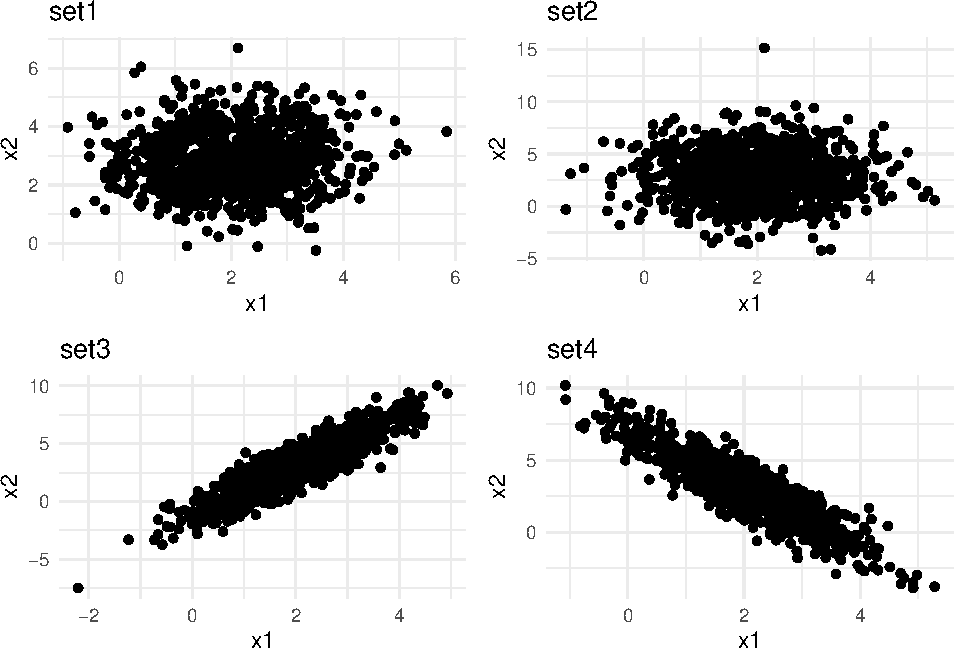
\includegraphics{RecEx2-sol_files/figure-latex/unnamed-chunk-11-1.pdf}

\section{Problem 6}\label{problem-6}

\subsection{a)}\label{a}

We sample from the model \(y=x^2+\epsilon\) where
\(\epsilon \sim \mathcal{N}(0,2^2)\) and
\(x\in \{-2,-1.9,-1.8,...,3.8,3.9,4\}\). This means that
\(y \sim \mathcal{N}(x^2,2^2)\). A total of 100 samples from this model
are generated for each of the 61 \(x\)'s.

See comments in code for further explanations.

\begin{Shaded}
\begin{Highlighting}[]
\KeywordTok{library}\NormalTok{(ggplot2)}
\KeywordTok{library}\NormalTok{(ggpubr)}
\KeywordTok{set.seed}\NormalTok{(}\DecValTok{2}\NormalTok{) }\CommentTok{# to reproduce}

\NormalTok{M=}\DecValTok{100} \CommentTok{# repeated samplings, x fixed }
\NormalTok{nord=}\DecValTok{20} \CommentTok{# order of polynoms}


\NormalTok{x =}\StringTok{ }\KeywordTok{seq}\NormalTok{(}\OperatorTok{-}\DecValTok{2}\NormalTok{, }\DecValTok{4}\NormalTok{, }\FloatTok{0.1}\NormalTok{) }\CommentTok{#We make a sequence of 61 points, x. These are the points for which we evaluate the function f(x).}
\NormalTok{truefunc=}\ControlFlowTok{function}\NormalTok{(x)\{}
  \KeywordTok{return}\NormalTok{(x}\OperatorTok{^}\DecValTok{2}\NormalTok{) }\CommentTok{#The true f(x)=x^2. }
\NormalTok{\}}
\NormalTok{true_y =}\StringTok{ }\KeywordTok{truefunc}\NormalTok{(x) }\CommentTok{#We find f(x) for each element in vector x.}

\NormalTok{error =}\StringTok{ }\KeywordTok{matrix}\NormalTok{(}\KeywordTok{rnorm}\NormalTok{(}\KeywordTok{length}\NormalTok{(x)}\OperatorTok{*}\NormalTok{M, }\DataTypeTok{mean=}\DecValTok{0}\NormalTok{, }\DataTypeTok{sd=}\DecValTok{2}\NormalTok{),}\DataTypeTok{nrow=}\NormalTok{M,}\DataTypeTok{byrow=}\OtherTok{TRUE}\NormalTok{) }\CommentTok{#Noise (epsilon) is sampled from a normal distribution and stored in this matrix. Each column corresponds to one value of x.}
\NormalTok{ymat =}\StringTok{ }\KeywordTok{matrix}\NormalTok{(}\KeywordTok{rep}\NormalTok{(true_y,M),}\DataTypeTok{byrow=}\NormalTok{T,}\DataTypeTok{nrow=}\NormalTok{M) }\OperatorTok{+}\StringTok{ }\NormalTok{error }\CommentTok{#The 100 samples or the observations are stored in this matrix.}

\NormalTok{predarray=}\KeywordTok{array}\NormalTok{(}\OtherTok{NA}\NormalTok{,}\DataTypeTok{dim=}\KeywordTok{c}\NormalTok{(M,}\KeywordTok{length}\NormalTok{(x),nord))}
\ControlFlowTok{for}\NormalTok{ (i }\ControlFlowTok{in} \DecValTok{1}\OperatorTok{:}\NormalTok{M)\{}
  \ControlFlowTok{for}\NormalTok{ (j }\ControlFlowTok{in} \DecValTok{1}\OperatorTok{:}\NormalTok{nord)\{}
\NormalTok{    predarray[i,,j]=}\KeywordTok{predict}\NormalTok{(}\KeywordTok{lm}\NormalTok{(ymat[i,]}\OperatorTok{~}\KeywordTok{poly}\NormalTok{(x, j,}\DataTypeTok{raw=}\OtherTok{TRUE}\NormalTok{)))}
    \CommentTok{#Based on the response y_i and the x_i's, we fit a polynomial model of degre 1,...,20. This means that we assume y_i~Normal(x_i^j,0). }
\NormalTok{  \}}
\NormalTok{\}}
\CommentTok{# M matrices of size length(x) times nord}
\CommentTok{# first, only look at variablity in the M fits and plot M curves where we had 1.}

\CommentTok{# for plotting need to stack the matrices underneath eachother and make new variable "rep"}
\NormalTok{stackmat=}\OtherTok{NULL}
\ControlFlowTok{for}\NormalTok{ (i }\ControlFlowTok{in} \DecValTok{1}\OperatorTok{:}\NormalTok{M) stackmat=}\KeywordTok{rbind}\NormalTok{(stackmat,}\KeywordTok{cbind}\NormalTok{(x,}\KeywordTok{rep}\NormalTok{(i,}\KeywordTok{length}\NormalTok{(x)),predarray[i,,]))}
\CommentTok{#dim(stackmat)}
\KeywordTok{colnames}\NormalTok{(stackmat)=}\KeywordTok{c}\NormalTok{(}\StringTok{"x"}\NormalTok{,}\StringTok{"rep"}\NormalTok{,}\KeywordTok{paste}\NormalTok{(}\StringTok{"poly"}\NormalTok{,}\DecValTok{1}\OperatorTok{:}\DecValTok{20}\NormalTok{,}\DataTypeTok{sep=}\StringTok{""}\NormalTok{))}
\NormalTok{sdf=}\KeywordTok{as.data.frame}\NormalTok{(stackmat) }\CommentTok{#NB have poly1-20 now - but first only use 1,2,20}
\CommentTok{# to add true curve using stat_function - easiest solution}
\NormalTok{true_x=x}
\NormalTok{yrange=}\KeywordTok{range}\NormalTok{(}\KeywordTok{apply}\NormalTok{(sdf,}\DecValTok{2}\NormalTok{,range)[,}\DecValTok{3}\OperatorTok{:}\DecValTok{22}\NormalTok{])}
\NormalTok{p1=}\KeywordTok{ggplot}\NormalTok{(}\DataTypeTok{data=}\NormalTok{sdf,}\KeywordTok{aes}\NormalTok{(}\DataTypeTok{x=}\NormalTok{x,}\DataTypeTok{y=}\NormalTok{poly1,}\DataTypeTok{group=}\NormalTok{rep,}\DataTypeTok{colour=}\NormalTok{rep))}\OperatorTok{+}\KeywordTok{scale_y_continuous}\NormalTok{(}\DataTypeTok{limits=}\NormalTok{yrange)}\OperatorTok{+}\KeywordTok{geom_line}\NormalTok{()}
\NormalTok{p1=p1}\OperatorTok{+}\KeywordTok{stat_function}\NormalTok{(}\DataTypeTok{fun=}\NormalTok{truefunc,}\DataTypeTok{lwd=}\FloatTok{1.3}\NormalTok{,}\DataTypeTok{colour=}\StringTok{"black"}\NormalTok{)}\OperatorTok{+}\KeywordTok{ggtitle}\NormalTok{(}\StringTok{"poly1"}\NormalTok{)}\OperatorTok{+}\KeywordTok{theme_minimal}\NormalTok{()}
\NormalTok{p2=}\KeywordTok{ggplot}\NormalTok{(}\DataTypeTok{data=}\NormalTok{sdf,}\KeywordTok{aes}\NormalTok{(}\DataTypeTok{x=}\NormalTok{x,}\DataTypeTok{y=}\NormalTok{poly2,}\DataTypeTok{group=}\NormalTok{rep,}\DataTypeTok{colour=}\NormalTok{rep))}\OperatorTok{+}\KeywordTok{scale_y_continuous}\NormalTok{(}\DataTypeTok{limits=}\NormalTok{yrange)}\OperatorTok{+}\KeywordTok{geom_line}\NormalTok{()}
\NormalTok{p2=p2}\OperatorTok{+}\KeywordTok{stat_function}\NormalTok{(}\DataTypeTok{fun=}\NormalTok{truefunc,}\DataTypeTok{lwd=}\FloatTok{1.3}\NormalTok{,}\DataTypeTok{colour=}\StringTok{"black"}\NormalTok{)}\OperatorTok{+}\KeywordTok{ggtitle}\NormalTok{(}\StringTok{"poly2"}\NormalTok{)}\OperatorTok{+}\KeywordTok{theme_minimal}\NormalTok{()}
\NormalTok{p10=}\KeywordTok{ggplot}\NormalTok{(}\DataTypeTok{data=}\NormalTok{sdf,}\KeywordTok{aes}\NormalTok{(}\DataTypeTok{x=}\NormalTok{x,}\DataTypeTok{y=}\NormalTok{poly10,}\DataTypeTok{group=}\NormalTok{rep,}\DataTypeTok{colour=}\NormalTok{rep))}\OperatorTok{+}\KeywordTok{scale_y_continuous}\NormalTok{(}\DataTypeTok{limits=}\NormalTok{yrange)}\OperatorTok{+}\KeywordTok{geom_line}\NormalTok{()}
\NormalTok{p10=p10}\OperatorTok{+}\KeywordTok{stat_function}\NormalTok{(}\DataTypeTok{fun=}\NormalTok{truefunc,}\DataTypeTok{lwd=}\FloatTok{1.3}\NormalTok{,}\DataTypeTok{colour=}\StringTok{"black"}\NormalTok{)}\OperatorTok{+}\KeywordTok{ggtitle}\NormalTok{(}\StringTok{"poly10"}\NormalTok{)}\OperatorTok{+}\KeywordTok{theme_minimal}\NormalTok{()}
\NormalTok{p20=}\KeywordTok{ggplot}\NormalTok{(}\DataTypeTok{data=}\NormalTok{sdf,}\KeywordTok{aes}\NormalTok{(}\DataTypeTok{x=}\NormalTok{x,}\DataTypeTok{y=}\NormalTok{poly20,}\DataTypeTok{group=}\NormalTok{rep,}\DataTypeTok{colour=}\NormalTok{rep))}\OperatorTok{+}\KeywordTok{scale_y_continuous}\NormalTok{(}\DataTypeTok{limits=}\NormalTok{yrange)}\OperatorTok{+}\KeywordTok{geom_line}\NormalTok{()}
\NormalTok{p20=p20}\OperatorTok{+}\KeywordTok{stat_function}\NormalTok{(}\DataTypeTok{fun=}\NormalTok{truefunc,}\DataTypeTok{lwd=}\FloatTok{1.3}\NormalTok{,}\DataTypeTok{colour=}\StringTok{"black"}\NormalTok{)}\OperatorTok{+}\KeywordTok{ggtitle}\NormalTok{(}\StringTok{"poly20"}\NormalTok{)}\OperatorTok{+}\KeywordTok{theme_minimal}\NormalTok{()}
\KeywordTok{ggarrange}\NormalTok{(p1,p2,p10,p20)}
\end{Highlighting}
\end{Shaded}

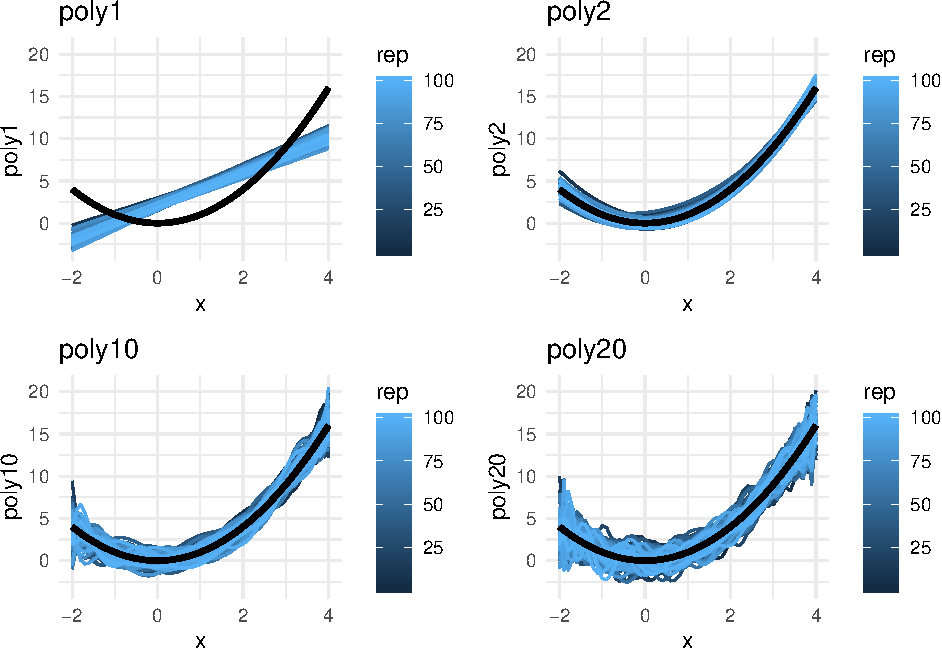
\includegraphics{RecEx2-sol_files/figure-latex/unnamed-chunk-12-1.pdf}

The upper left plot shows 100 predictions when we assume that \(y\) is a
linear function of \(x\), the upper right plot hows 100 predictions when
we assume that \(y\) is function of poynomials up to \(x^2\), the lower
left plot shows 100 predictions when we assume \(y\) is a function of
polynomials up to \(x^{10}\) and the lower right plot shows 100
predictions when assuming \(y\) is a function of polynomials up to
\(x^{20}\).

\subsection{b)}\label{b}

Run the code attached and consider the following plots:

\begin{Shaded}
\begin{Highlighting}[]
\KeywordTok{set.seed}\NormalTok{(}\DecValTok{2}\NormalTok{) }\CommentTok{# to reproduce}

\NormalTok{M=}\DecValTok{100} \CommentTok{# repeated samplings,x fixed but new errors}
\NormalTok{nord=}\DecValTok{20}
\NormalTok{x =}\StringTok{ }\KeywordTok{seq}\NormalTok{(}\OperatorTok{-}\DecValTok{2}\NormalTok{, }\DecValTok{4}\NormalTok{, }\FloatTok{0.1}\NormalTok{)}
\NormalTok{truefunc=}\ControlFlowTok{function}\NormalTok{(x) }\KeywordTok{return}\NormalTok{(x}\OperatorTok{^}\DecValTok{2}\NormalTok{)}
\NormalTok{true_y =}\StringTok{ }\KeywordTok{truefunc}\NormalTok{(x)}

\NormalTok{error =}\StringTok{ }\KeywordTok{matrix}\NormalTok{(}\KeywordTok{rnorm}\NormalTok{(}\KeywordTok{length}\NormalTok{(x)}\OperatorTok{*}\NormalTok{M, }\DataTypeTok{mean=}\DecValTok{0}\NormalTok{, }\DataTypeTok{sd=}\DecValTok{2}\NormalTok{),}\DataTypeTok{nrow=}\NormalTok{M,}\DataTypeTok{byrow=}\OtherTok{TRUE}\NormalTok{)}
\NormalTok{testerror =}\StringTok{ }\KeywordTok{matrix}\NormalTok{(}\KeywordTok{rnorm}\NormalTok{(}\KeywordTok{length}\NormalTok{(x)}\OperatorTok{*}\NormalTok{M, }\DataTypeTok{mean=}\DecValTok{0}\NormalTok{, }\DataTypeTok{sd=}\DecValTok{2}\NormalTok{),}\DataTypeTok{nrow=}\NormalTok{M,}\DataTypeTok{byrow=}\OtherTok{TRUE}\NormalTok{)}
\NormalTok{ymat =}\StringTok{ }\KeywordTok{matrix}\NormalTok{(}\KeywordTok{rep}\NormalTok{(true_y,M),}\DataTypeTok{byrow=}\NormalTok{T,}\DataTypeTok{nrow=}\NormalTok{M) }\OperatorTok{+}\StringTok{ }\NormalTok{error}
\NormalTok{testymat =}\StringTok{ }\KeywordTok{matrix}\NormalTok{(}\KeywordTok{rep}\NormalTok{(true_y,M),}\DataTypeTok{byrow=}\NormalTok{T,}\DataTypeTok{nrow=}\NormalTok{M) }\OperatorTok{+}\StringTok{ }\NormalTok{testerror}

\NormalTok{predarray=}\KeywordTok{array}\NormalTok{(}\OtherTok{NA}\NormalTok{,}\DataTypeTok{dim=}\KeywordTok{c}\NormalTok{(M,}\KeywordTok{length}\NormalTok{(x),nord))}
\ControlFlowTok{for}\NormalTok{ (i }\ControlFlowTok{in} \DecValTok{1}\OperatorTok{:}\NormalTok{M)}
\NormalTok{\{}
  \ControlFlowTok{for}\NormalTok{ (j }\ControlFlowTok{in} \DecValTok{1}\OperatorTok{:}\NormalTok{nord)}
\NormalTok{  \{}
\NormalTok{    predarray[i,,j]=}\KeywordTok{predict}\NormalTok{(}\KeywordTok{lm}\NormalTok{(ymat[i,]}\OperatorTok{~}\KeywordTok{poly}\NormalTok{(x, j,}\DataTypeTok{raw=}\OtherTok{TRUE}\NormalTok{)))}
\NormalTok{  \}}
\NormalTok{\}  }
\NormalTok{trainMSE=}\KeywordTok{matrix}\NormalTok{(}\DataTypeTok{ncol=}\NormalTok{nord,}\DataTypeTok{nrow=}\NormalTok{M)}
\ControlFlowTok{for}\NormalTok{ (i }\ControlFlowTok{in} \DecValTok{1}\OperatorTok{:}\NormalTok{M) trainMSE[i,]=}\KeywordTok{apply}\NormalTok{((predarray[i,,]}\OperatorTok{-}\NormalTok{ymat[i,])}\OperatorTok{^}\DecValTok{2}\NormalTok{,}\DecValTok{2}\NormalTok{,mean)}
\NormalTok{testMSE=}\KeywordTok{matrix}\NormalTok{(}\DataTypeTok{ncol=}\NormalTok{nord,}\DataTypeTok{nrow=}\NormalTok{M)}
\ControlFlowTok{for}\NormalTok{ (i }\ControlFlowTok{in} \DecValTok{1}\OperatorTok{:}\NormalTok{M) testMSE[i,]=}\KeywordTok{apply}\NormalTok{((predarray[i,,]}\OperatorTok{-}\NormalTok{testymat[i,])}\OperatorTok{^}\DecValTok{2}\NormalTok{,}\DecValTok{2}\NormalTok{,mean)}

\KeywordTok{library}\NormalTok{(ggplot2)}
\KeywordTok{library}\NormalTok{(ggpubr)}

\CommentTok{# format suitable for plotting }
\NormalTok{stackmat=}\OtherTok{NULL}
\ControlFlowTok{for}\NormalTok{ (i }\ControlFlowTok{in} \DecValTok{1}\OperatorTok{:}\NormalTok{M) stackmat=}\KeywordTok{rbind}\NormalTok{(stackmat,}\KeywordTok{cbind}\NormalTok{(}\KeywordTok{rep}\NormalTok{(i,nord),}\DecValTok{1}\OperatorTok{:}\NormalTok{nord,trainMSE[i,],testMSE[i,]))}
\KeywordTok{colnames}\NormalTok{(stackmat)=}\KeywordTok{c}\NormalTok{(}\StringTok{"rep"}\NormalTok{,}\StringTok{"poly"}\NormalTok{,}\StringTok{"trainMSE"}\NormalTok{,}\StringTok{"testMSE"}\NormalTok{)}
\NormalTok{sdf=}\KeywordTok{as.data.frame}\NormalTok{(stackmat) }
\NormalTok{yrange=}\KeywordTok{range}\NormalTok{(sdf[,}\DecValTok{3}\OperatorTok{:}\DecValTok{4}\NormalTok{])}
\NormalTok{p1=}\KeywordTok{ggplot}\NormalTok{(}\DataTypeTok{data=}\NormalTok{sdf[}\DecValTok{1}\OperatorTok{:}\NormalTok{nord,],}\KeywordTok{aes}\NormalTok{(}\DataTypeTok{x=}\NormalTok{poly,}\DataTypeTok{y=}\NormalTok{trainMSE))}\OperatorTok{+}\KeywordTok{scale_y_continuous}\NormalTok{(}\DataTypeTok{limits=}\NormalTok{yrange)}\OperatorTok{+}\KeywordTok{geom_line}\NormalTok{()}\OperatorTok{+}\KeywordTok{theme_minimal}\NormalTok{()}
\NormalTok{pall=}\StringTok{ }\KeywordTok{ggplot}\NormalTok{(}\DataTypeTok{data=}\NormalTok{sdf,}\KeywordTok{aes}\NormalTok{(}\DataTypeTok{x=}\NormalTok{poly,}\DataTypeTok{group=}\NormalTok{rep,}\DataTypeTok{y=}\NormalTok{trainMSE,}\DataTypeTok{colour=}\NormalTok{rep))}\OperatorTok{+}\KeywordTok{scale_y_continuous}\NormalTok{(}\DataTypeTok{limits=}\NormalTok{yrange)}\OperatorTok{+}\KeywordTok{geom_line}\NormalTok{()}\OperatorTok{+}\KeywordTok{theme_minimal}\NormalTok{()}
\NormalTok{testp1=}\KeywordTok{ggplot}\NormalTok{(}\DataTypeTok{data=}\NormalTok{sdf[}\DecValTok{1}\OperatorTok{:}\NormalTok{nord,],}\KeywordTok{aes}\NormalTok{(}\DataTypeTok{x=}\NormalTok{poly,}\DataTypeTok{y=}\NormalTok{testMSE))}\OperatorTok{+}\KeywordTok{scale_y_continuous}\NormalTok{(}\DataTypeTok{limits=}\NormalTok{yrange)}\OperatorTok{+}\KeywordTok{geom_line}\NormalTok{()}\OperatorTok{+}\KeywordTok{theme_minimal}\NormalTok{()}
\NormalTok{testpall=}\StringTok{ }\KeywordTok{ggplot}\NormalTok{(}\DataTypeTok{data=}\NormalTok{sdf,}\KeywordTok{aes}\NormalTok{(}\DataTypeTok{x=}\NormalTok{poly,}\DataTypeTok{group=}\NormalTok{rep,}\DataTypeTok{y=}\NormalTok{testMSE,}\DataTypeTok{colour=}\NormalTok{rep))}\OperatorTok{+}\KeywordTok{scale_y_continuous}\NormalTok{(}\DataTypeTok{limits=}\NormalTok{yrange)}\OperatorTok{+}\KeywordTok{geom_line}\NormalTok{()}\OperatorTok{+}\KeywordTok{theme_minimal}\NormalTok{()}
\KeywordTok{ggarrange}\NormalTok{(p1,pall,testp1,testpall)}
\end{Highlighting}
\end{Shaded}

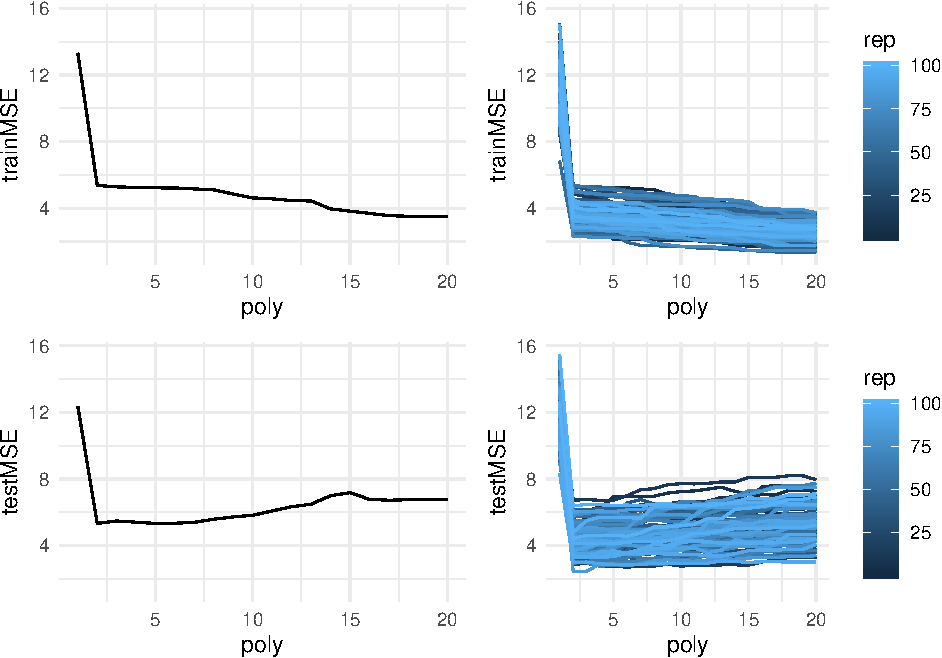
\includegraphics{RecEx2-sol_files/figure-latex/unnamed-chunk-13-1.pdf}

\begin{Shaded}
\begin{Highlighting}[]
\KeywordTok{library}\NormalTok{(reshape2)}
\NormalTok{df=}\KeywordTok{melt}\NormalTok{(sdf,}\DataTypeTok{id=}\KeywordTok{c}\NormalTok{(}\StringTok{"poly"}\NormalTok{,}\StringTok{"rep"}\NormalTok{))[,}\OperatorTok{-}\DecValTok{2}\NormalTok{]}
\KeywordTok{colnames}\NormalTok{(df)[}\DecValTok{2}\NormalTok{]=}\StringTok{"MSEtype"}
\KeywordTok{ggplot}\NormalTok{(}\DataTypeTok{data=}\NormalTok{df,}\KeywordTok{aes}\NormalTok{(}\DataTypeTok{x=}\KeywordTok{as.factor}\NormalTok{(poly),}\DataTypeTok{y=}\NormalTok{value))}\OperatorTok{+}\KeywordTok{geom_boxplot}\NormalTok{(}\KeywordTok{aes}\NormalTok{(}\DataTypeTok{fill=}\NormalTok{MSEtype))}
\end{Highlighting}
\end{Shaded}

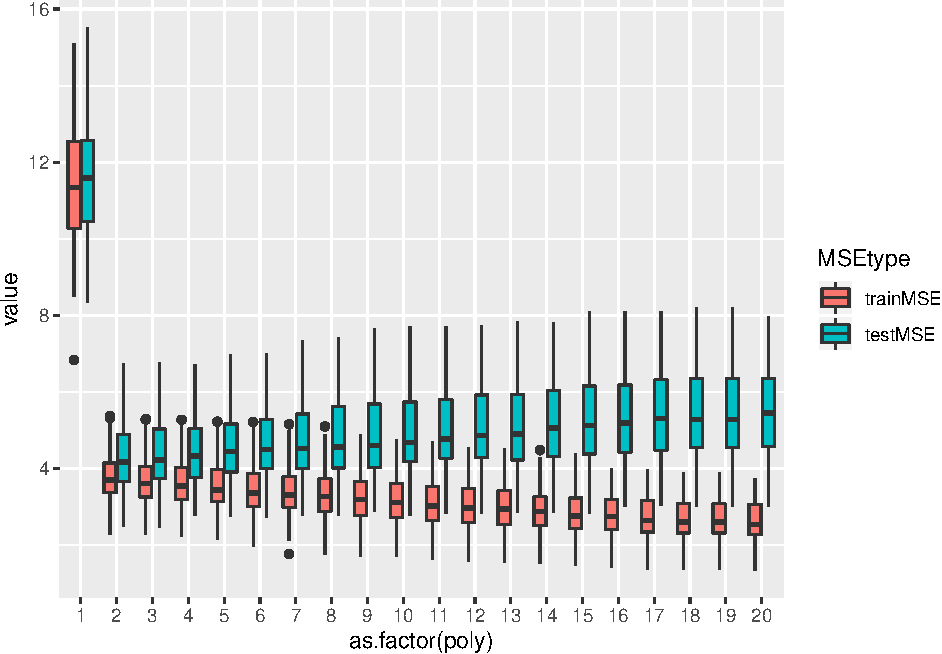
\includegraphics{RecEx2-sol_files/figure-latex/unnamed-chunk-13-2.pdf}

\begin{Shaded}
\begin{Highlighting}[]
\NormalTok{trainMSEmean=}\KeywordTok{apply}\NormalTok{(trainMSE,}\DecValTok{2}\NormalTok{,mean)}
\NormalTok{testMSEmean=}\KeywordTok{apply}\NormalTok{(testMSE,}\DecValTok{2}\NormalTok{,mean)}
\NormalTok{meandf=}\KeywordTok{melt}\NormalTok{(}\KeywordTok{data.frame}\NormalTok{(}\KeywordTok{cbind}\NormalTok{(}\StringTok{"poly"}\NormalTok{=}\DecValTok{1}\OperatorTok{:}\NormalTok{nord,trainMSEmean,testMSEmean)),}\DataTypeTok{id=}\StringTok{"poly"}\NormalTok{)}
\KeywordTok{ggplot}\NormalTok{(}\DataTypeTok{data=}\NormalTok{meandf,}\KeywordTok{aes}\NormalTok{(}\DataTypeTok{x=}\NormalTok{poly,}\DataTypeTok{y=}\NormalTok{value,}\DataTypeTok{colour=}\NormalTok{variable))}\OperatorTok{+}\KeywordTok{geom_line}\NormalTok{()}\OperatorTok{+}\KeywordTok{theme_minimal}\NormalTok{()}
\end{Highlighting}
\end{Shaded}

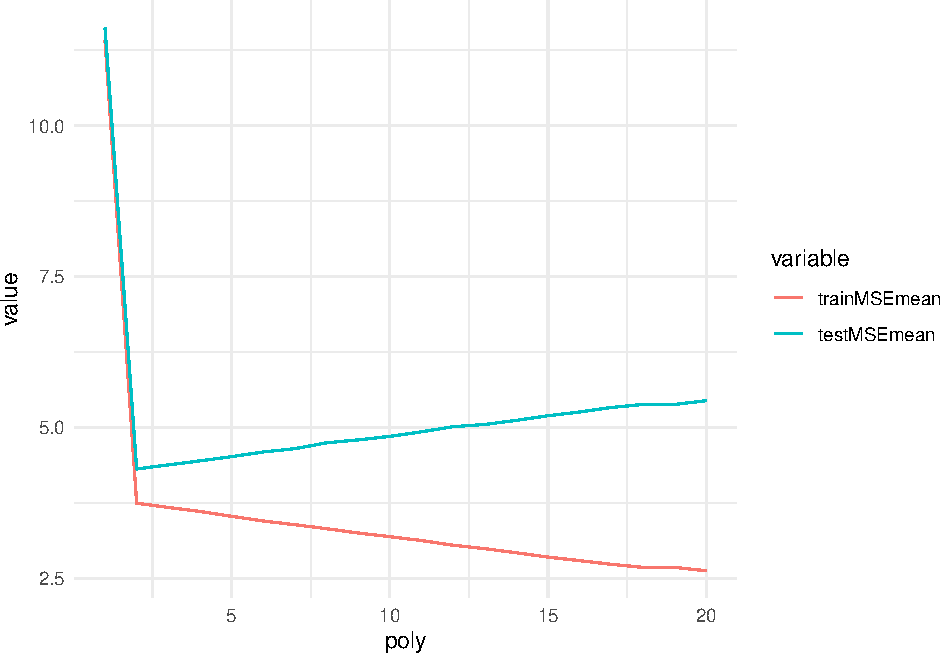
\includegraphics{RecEx2-sol_files/figure-latex/unnamed-chunk-13-3.pdf}

The plots show that the test MSE in general is larger than the train
MSE. This is reasonable. The fitted model is fitted based on the
training set. Thus, the error will be smaller for the train data than
for the test data. Furthermore, the plots show that the difference
between the MSE for the test set and the training set increases when the
degree of the polynomial increases. When the degree of the polynomial
increases, we get a more flexible model. The fitted curve will try to
pass through the training data if possible, which typically leads to an
overfitted model that performs bad for test data.

\begin{itemize}
\tightlist
\item
  We observe that poly 2 gives the smallest mean testMSE, while poly 20
  gives the smallest trainMSE. Based on these plots, we would choose
  poly 2 for prediction of a new value of \(y\), as the testMSE tells us
  more about how the model performs on data not used to train the model.
\end{itemize}

\subsection{c)}\label{c}

Run the code and consider the following plots:

\begin{Shaded}
\begin{Highlighting}[]
\NormalTok{meanmat=}\KeywordTok{matrix}\NormalTok{(}\DataTypeTok{ncol=}\KeywordTok{length}\NormalTok{(x),}\DataTypeTok{nrow=}\NormalTok{nord)}
\NormalTok{varmat=}\KeywordTok{matrix}\NormalTok{(}\DataTypeTok{ncol=}\KeywordTok{length}\NormalTok{(x),}\DataTypeTok{nrow=}\NormalTok{nord)}
\ControlFlowTok{for}\NormalTok{ (j }\ControlFlowTok{in} \DecValTok{1}\OperatorTok{:}\NormalTok{nord)}
\NormalTok{\{}
\NormalTok{  meanmat[j,]=}\KeywordTok{apply}\NormalTok{(predarray[,,j],}\DecValTok{2}\NormalTok{,mean) }\CommentTok{# we now take the mean over the M simulations - to mimic E and Var at each x value and each poly model}
\NormalTok{  varmat[j,]=}\KeywordTok{apply}\NormalTok{(predarray[,,j],}\DecValTok{2}\NormalTok{,var)}
\NormalTok{\}}
\CommentTok{# nord times length(x)}
\NormalTok{bias2mat=(meanmat}\OperatorTok{-}\KeywordTok{matrix}\NormalTok{(}\KeywordTok{rep}\NormalTok{(true_y,nord),}\DataTypeTok{byrow=}\OtherTok{TRUE}\NormalTok{,}\DataTypeTok{nrow=}\NormalTok{nord))}\OperatorTok{^}\DecValTok{2} \CommentTok{#here the truth is}

\NormalTok{df=}\KeywordTok{data.frame}\NormalTok{(}\KeywordTok{rep}\NormalTok{(x,}\DataTypeTok{each=}\NormalTok{nord),}\KeywordTok{rep}\NormalTok{(}\DecValTok{1}\OperatorTok{:}\NormalTok{nord,}\KeywordTok{length}\NormalTok{(x)),}\KeywordTok{c}\NormalTok{(bias2mat),}\KeywordTok{c}\NormalTok{(varmat),}\KeywordTok{rep}\NormalTok{(}\DecValTok{4}\NormalTok{,}\KeywordTok{prod}\NormalTok{(}\KeywordTok{dim}\NormalTok{(varmat)))) }\CommentTok{#irr is 2^2.}
\KeywordTok{colnames}\NormalTok{(df)=}\KeywordTok{c}\NormalTok{(}\StringTok{"x"}\NormalTok{,}\StringTok{"poly"}\NormalTok{,}\StringTok{"bias2"}\NormalTok{,}\StringTok{"variance"}\NormalTok{,}\StringTok{"irreducible error"}\NormalTok{) }\CommentTok{#suitable for plotting}
\NormalTok{df}\OperatorTok{$}\NormalTok{total=df}\OperatorTok{$}\NormalTok{bias2}\OperatorTok{+}\NormalTok{df}\OperatorTok{$}\NormalTok{variance}\OperatorTok{+}\NormalTok{df}\OperatorTok{$}\StringTok{`}\DataTypeTok{irreducible error}\StringTok{`}
\NormalTok{hdf=}\KeywordTok{melt}\NormalTok{(df,}\DataTypeTok{id=}\KeywordTok{c}\NormalTok{(}\StringTok{"x"}\NormalTok{,}\StringTok{"poly"}\NormalTok{))}
\NormalTok{hdf1=hdf[hdf}\OperatorTok{$}\NormalTok{poly}\OperatorTok{==}\DecValTok{1}\NormalTok{,]}
\NormalTok{hdf2=hdf[hdf}\OperatorTok{$}\NormalTok{poly}\OperatorTok{==}\DecValTok{2}\NormalTok{,]}
\NormalTok{hdf10=hdf[hdf}\OperatorTok{$}\NormalTok{poly}\OperatorTok{==}\DecValTok{10}\NormalTok{,]}
\NormalTok{hdf20=hdf[hdf}\OperatorTok{$}\NormalTok{poly}\OperatorTok{==}\DecValTok{20}\NormalTok{,]}

\NormalTok{p1=}\KeywordTok{ggplot}\NormalTok{(}\DataTypeTok{data=}\NormalTok{hdf1,}\KeywordTok{aes}\NormalTok{(}\DataTypeTok{x=}\NormalTok{x,}\DataTypeTok{y=}\NormalTok{value,}\DataTypeTok{colour=}\NormalTok{variable))}\OperatorTok{+}\KeywordTok{geom_line}\NormalTok{()}\OperatorTok{+}\KeywordTok{ggtitle}\NormalTok{(}\StringTok{"poly1"}\NormalTok{)}\OperatorTok{+}\KeywordTok{theme_minimal}\NormalTok{()}
\NormalTok{p2=}\KeywordTok{ggplot}\NormalTok{(}\DataTypeTok{data=}\NormalTok{hdf2,}\KeywordTok{aes}\NormalTok{(}\DataTypeTok{x=}\NormalTok{x,}\DataTypeTok{y=}\NormalTok{value,}\DataTypeTok{colour=}\NormalTok{variable))}\OperatorTok{+}\KeywordTok{geom_line}\NormalTok{()}\OperatorTok{+}\KeywordTok{ggtitle}\NormalTok{(}\StringTok{"poly2"}\NormalTok{)}\OperatorTok{+}\KeywordTok{theme_minimal}\NormalTok{()}
\NormalTok{p10=}\KeywordTok{ggplot}\NormalTok{(}\DataTypeTok{data=}\NormalTok{hdf10,}\KeywordTok{aes}\NormalTok{(}\DataTypeTok{x=}\NormalTok{x,}\DataTypeTok{y=}\NormalTok{value,}\DataTypeTok{colour=}\NormalTok{variable))}\OperatorTok{+}\KeywordTok{geom_line}\NormalTok{()}\OperatorTok{+}\KeywordTok{ggtitle}\NormalTok{(}\StringTok{"poly10"}\NormalTok{)}\OperatorTok{+}\KeywordTok{theme_minimal}\NormalTok{()}
\NormalTok{p20=}\KeywordTok{ggplot}\NormalTok{(}\DataTypeTok{data=}\NormalTok{hdf20,}\KeywordTok{aes}\NormalTok{(}\DataTypeTok{x=}\NormalTok{x,}\DataTypeTok{y=}\NormalTok{value,}\DataTypeTok{colour=}\NormalTok{variable))}\OperatorTok{+}\KeywordTok{geom_line}\NormalTok{()}\OperatorTok{+}\KeywordTok{ggtitle}\NormalTok{(}\StringTok{"poly20"}\NormalTok{)}\OperatorTok{+}\KeywordTok{theme_minimal}\NormalTok{()}
\KeywordTok{ggarrange}\NormalTok{(p1,p2,p10,p20)}
\end{Highlighting}
\end{Shaded}

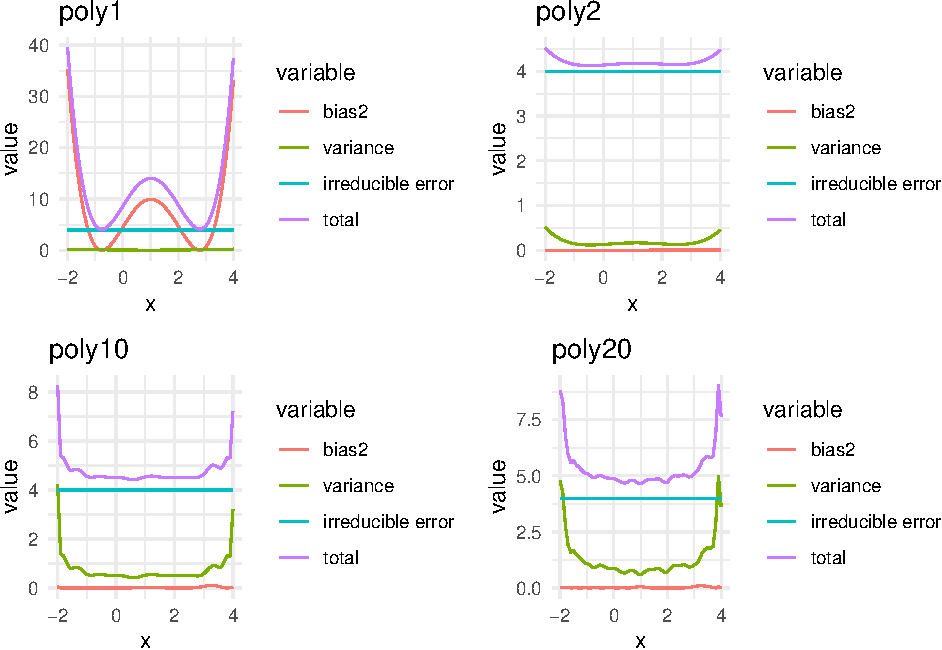
\includegraphics{RecEx2-sol_files/figure-latex/unnamed-chunk-14-1.pdf}

We see that the irriducible error remains constant with the complexity
of the model and the variance (green) increases with the complexity. A
linear model gives variance close to zero, while a polynomial of degree
20 gives variance close to 1 (larger at the borders). A more complex
model is more flexible as it can turn up and down and change direction
fast. This leads to larger variance. (Look at the plot in 2a, there is a
larger variety of curves you can make when the degree is 20 compared to
if the degree is 1.).

Further, we see that the bias is large for poly1, the linear model. The
linear model is quite rigid, so if the true underlying model is
non-linear, we typically get large deviations between the fitted line
and the training data. If we study the first plot, it seems like the
fitted line goes through the training data in \(x=-1\) and \(x=3\) as
the bias is close to zero here (this is confirmed by looking at the
upper left plot in 2a).

The polynomial models with degree larger than one lead to lower bias.
Recall that this is the training bias: The polynomial models will try to
pass through the training points if possible, and when the degree of the
polynomial is large they are able to do so because they have large
flexibility compared to a linear model.

\begin{Shaded}
\begin{Highlighting}[]
\NormalTok{hdfatxa=hdf[hdf}\OperatorTok{$}\NormalTok{x}\OperatorTok{==-}\DecValTok{1}\NormalTok{,]}
\NormalTok{hdfatxb=hdf[hdf}\OperatorTok{$}\NormalTok{x}\OperatorTok{==}\FloatTok{0.5}\NormalTok{,]}
\NormalTok{hdfatxc=hdf[hdf}\OperatorTok{$}\NormalTok{x}\OperatorTok{==}\DecValTok{2}\NormalTok{,]}
\NormalTok{hdfatxd=hdf[hdf}\OperatorTok{$}\NormalTok{x}\OperatorTok{==}\FloatTok{3.5}\NormalTok{,]}
\NormalTok{pa=}\KeywordTok{ggplot}\NormalTok{(}\DataTypeTok{data=}\NormalTok{hdfatxa,}\KeywordTok{aes}\NormalTok{(}\DataTypeTok{x=}\NormalTok{poly,}\DataTypeTok{y=}\NormalTok{value,}\DataTypeTok{colour=}\NormalTok{variable))}\OperatorTok{+}\KeywordTok{geom_line}\NormalTok{()}\OperatorTok{+}\KeywordTok{ggtitle}\NormalTok{(}\StringTok{"x0=-1"}\NormalTok{)}\OperatorTok{+}\KeywordTok{theme_minimal}\NormalTok{()}
\NormalTok{pb=}\KeywordTok{ggplot}\NormalTok{(}\DataTypeTok{data=}\NormalTok{hdfatxb,}\KeywordTok{aes}\NormalTok{(}\DataTypeTok{x=}\NormalTok{poly,}\DataTypeTok{y=}\NormalTok{value,}\DataTypeTok{colour=}\NormalTok{variable))}\OperatorTok{+}\KeywordTok{geom_line}\NormalTok{()}\OperatorTok{+}\KeywordTok{ggtitle}\NormalTok{(}\StringTok{"x0=0.5"}\NormalTok{)}\OperatorTok{+}\KeywordTok{theme_minimal}\NormalTok{()}
\NormalTok{pc=}\KeywordTok{ggplot}\NormalTok{(}\DataTypeTok{data=}\NormalTok{hdfatxc,}\KeywordTok{aes}\NormalTok{(}\DataTypeTok{x=}\NormalTok{poly,}\DataTypeTok{y=}\NormalTok{value,}\DataTypeTok{colour=}\NormalTok{variable))}\OperatorTok{+}\KeywordTok{geom_line}\NormalTok{()}\OperatorTok{+}\KeywordTok{ggtitle}\NormalTok{(}\StringTok{"x0=2"}\NormalTok{)}\OperatorTok{+}\KeywordTok{theme_minimal}\NormalTok{()}
\NormalTok{pd=}\KeywordTok{ggplot}\NormalTok{(}\DataTypeTok{data=}\NormalTok{hdfatxd,}\KeywordTok{aes}\NormalTok{(}\DataTypeTok{x=}\NormalTok{poly,}\DataTypeTok{y=}\NormalTok{value,}\DataTypeTok{colour=}\NormalTok{variable))}\OperatorTok{+}\KeywordTok{geom_line}\NormalTok{()}\OperatorTok{+}\KeywordTok{ggtitle}\NormalTok{(}\StringTok{"x0=3.5"}\NormalTok{)}\OperatorTok{+}\KeywordTok{theme_minimal}\NormalTok{()}
\KeywordTok{ggarrange}\NormalTok{(pa,pb,pc,pd)}
\end{Highlighting}
\end{Shaded}

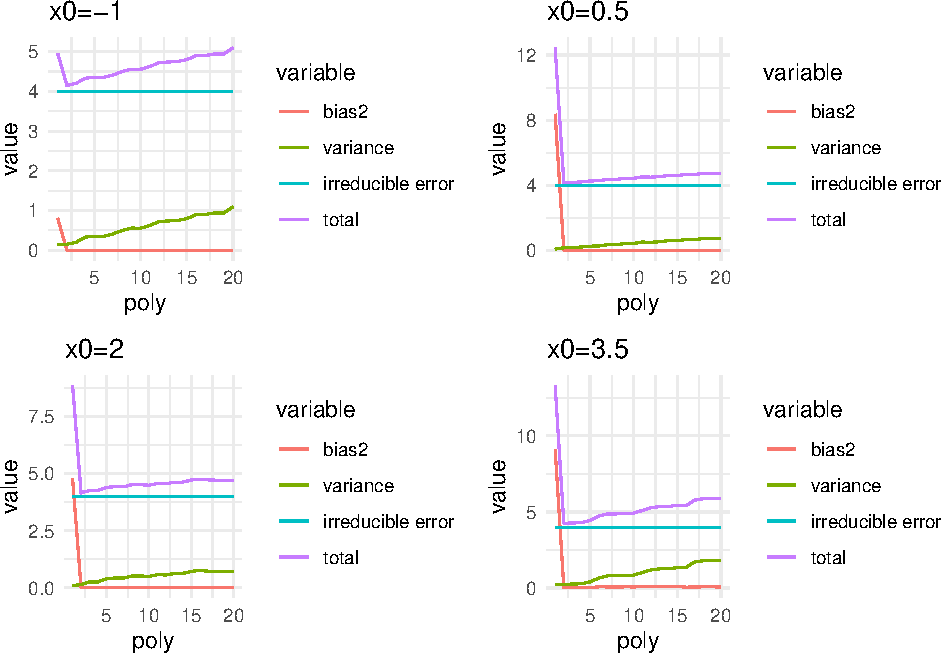
\includegraphics{RecEx2-sol_files/figure-latex/2bbiasvariance2-1.pdf}

Compare to Figures in 2.12 on page 36 in ISL (our textbook).

\subsection{d)}\label{d}

To change \(f(x)\), replace

\begin{Shaded}
\begin{Highlighting}[]
\NormalTok{truefunc=}\ControlFlowTok{function}\NormalTok{(x) }\KeywordTok{return}\NormalTok{(x}\OperatorTok{^}\DecValTok{2}\NormalTok{)}
\end{Highlighting}
\end{Shaded}

by for example

\begin{Shaded}
\begin{Highlighting}[]
\NormalTok{truefunc=}\ControlFlowTok{function}\NormalTok{(x) }\KeywordTok{return}\NormalTok{(x}\OperatorTok{^}\DecValTok{4}\NormalTok{)}
\end{Highlighting}
\end{Shaded}

or

\begin{Shaded}
\begin{Highlighting}[]
\NormalTok{truefunc=}\ControlFlowTok{function}\NormalTok{(x) }\KeywordTok{return}\NormalTok{(}\KeywordTok{exp}\NormalTok{(}\DecValTok{2}\OperatorTok{*}\NormalTok{x))}
\end{Highlighting}
\end{Shaded}

and rerun the code. Study the results.

If you want to set the variance to 1 for example, set \(sd=1\) in these
parts of the code in 2a and 2b:

\begin{verbatim}
rnorm(length(x)*M, mean=0, sd=1)
\end{verbatim}

Also change the following part in 2c:

\begin{Shaded}
\begin{Highlighting}[]
\NormalTok{df=}\KeywordTok{data.frame}\NormalTok{(}\KeywordTok{rep}\NormalTok{(x,}\DataTypeTok{each=}\NormalTok{nord),}\KeywordTok{rep}\NormalTok{(}\DecValTok{1}\OperatorTok{:}\NormalTok{nord,}\KeywordTok{length}\NormalTok{(x)),}\KeywordTok{c}\NormalTok{(bias2mat),}\KeywordTok{c}\NormalTok{(varmat),}\KeywordTok{rep}\NormalTok{(}\DecValTok{1}\NormalTok{,}\KeywordTok{prod}\NormalTok{(}\KeywordTok{dim}\NormalTok{(varmat)))) }\CommentTok{#irr is 1^2.}
\end{Highlighting}
\end{Shaded}

to get correct plots of the irreducible error. Here,
\(rep(4,prod(dim(varmat)))\) is replaced by
\(rep(1,prod(dim(varmat)))\).

\section{ R packages}\label{r-packages}

If you want to look at the .Rmd file and \texttt{knit} it, you need to
first install the following packages (only once).

\begin{Shaded}
\begin{Highlighting}[]
\KeywordTok{install.packages}\NormalTok{(}\StringTok{"ggplot2"}\NormalTok{)}
\KeywordTok{install.packages}\NormalTok{(}\StringTok{"gamlss.data"}\NormalTok{)}
\KeywordTok{install.packages}\NormalTok{(}\StringTok{"tidyverse"}\NormalTok{)}
\KeywordTok{install.packages}\NormalTok{(}\StringTok{"GGally"}\NormalTok{)}
\KeywordTok{install.packages}\NormalTok{(}\StringTok{"Matrix"}\NormalTok{)}
\KeywordTok{install.packages}\NormalTok{(}\StringTok{"ggpubr"}\NormalTok{)}
\end{Highlighting}
\end{Shaded}


\end{document}
